\documentclass[12pt,a4paper,oneside]{article}
\usepackage{amsfonts, amsmath, amssymb,latexsym,amsthm}
\usepackage[english]{babel}
\usepackage{epsfig}
\usepackage{enumerate}
\usepackage{graphicx} 
\usepackage{float}
\usepackage{subfigure}
\usepackage{cancel}
\usepackage{feynmf}
\usepackage[table,xcdraw]{xcolor}

\numberwithin{equation}{section}

\parskip=5pt
\parindent=15pt

\usepackage[left=1.7cm,top=2.7cm,right=1.7cm,bottom=2.7cm]{geometry}

\usepackage[utf8]{inputenc}
\usepackage{ dsfont }

\setcounter{page}{1}

\numberwithin{equation}{section}
\newtheorem{question}{Question}
\newtheorem{teorema}{Teorema}
\newtheorem{proposicio}{Proposici\'{o}}
\newtheorem{corollari}{Corol$\cdot$lari}
\newtheorem{lema}{Lema}

\theoremstyle{definition}
\newtheorem{remark}{Remark}
\newtheorem{exercici}{Exercise}
\newtheorem{problema}{Problem}
\newtheorem*{solucio}{Solution}
\newtheorem{exemple}{Exemple}
\newtheorem{exemples}{Exemples}
\newtheorem{observacio}{Observaci\'{o}}
\newtheorem{observacions}{Observacions}
\newcommand{\Q}{\mathds{Q}}
\newcommand{\A}{\alpha}
\newcommand{\C}{\mathds{C}}
\newcommand{\Z}{\mathds{Z}}
\newcommand{\R}{\mathds{R}}
\newcommand{\N}{\mathds{N}}
\newcommand{\F}{\mathds{F}}
\newcommand{\B}{\mathcal{B}}
\newcommand{\Irr}{\mbox{Irr}}
\newcommand{\gr}{\mbox{gr}}
\newcommand{\Gal}{\mbox{Gal}}

\def\qed{\hfill $\square$}

\usepackage{fancyhdr}

\pagestyle{fancy}

\lhead{Jorge Rodr\'{i}guez Molinuevo}
\chead{}
\rhead{Complex Networks $ 1^{st} $ activity}

\cfoot{\thepage}

\bibstyle{plain}
\date{\today}

\begin{document}

% PORTADA
\begin{center}
	\textbf{ }\\[4cm]
	
	\LARGE First Laboratory\\[0.5cm]
	\textbf{{\Huge Structural descriptors of complex networks}}\\[0.5cm]
	\textbf{{\LARGE Complex Networks}}\\[1.5cm]
	
	{\Large Universitat Rovira i Virgili}\\[2.3cm]
	{\LARGE \textbf{Master in Artificial Inteligence}}\\[0.5cm]
	{\LARGE $2^{nd}$ Semester}\\[2.5cm]
	
	\begin{flushright}
		\textbf{\large{Author:}\\ \normalsize{Jorge Rodriguez Molinuevo\\}}
	\end{flushright}
	\today
\end{center}
\thispagestyle{empty} 
%\maketitle

\pagebreak

\section{Calculation of structural descriptors of complex networks}

\subsection{Numerical descriptors}
\begin{table}[h!]
	\centering
	\caption{Table for the structural descriptors}
	\label{table}
	\tabcolsep=0.11cm
	\small
	\begin{tabular}{l|lllllll}
		\multicolumn{1}{c|}{Networks} & \multicolumn{1}{c}{\begin{tabular}[c]{@{}c@{}}Number \\ of \\ Nodes\end{tabular}} & \multicolumn{1}{c}{\begin{tabular}[c]{@{}c@{}}Number \\ of \\ Edges\end{tabular}} & \multicolumn{1}{c}{\begin{tabular}[c]{@{}c@{}}Average , \\ maximum and\\ minimum degree\end{tabular}} & \multicolumn{1}{c}{\begin{tabular}[c]{@{}c@{}}Average \\ clustering\\ coefficient\end{tabular}} & \multicolumn{1}{c}{Assortativity} & \multicolumn{1}{c}{\begin{tabular}[c]{@{}c@{}}Average \\ path\\ length\end{tabular}} & \multicolumn{1}{c}{Diameter} \\ \hline
		20x2+5x2 &50 &404 &16.16,22,4 &0.9716 &0.9186 &3 &5 \\ 
		circle9 &9 &9 &2.0,2,2 &0.0 &nan &3 &5 \\
		graph3+1+3 &7 &8 &2.2857,3,2 &0.6667 &-0.6 &3 &5 \\
		graph3+2+3 &8 &13 &3.25,4,3 &0.875 &-0.0833 &2 &4 \\ 
		grid-p-6x6 &36 &72 &4.0,4,4 &0.0 &nan &4 &7 \\ 
		rb25 &25 &66 &5.28,20,4 &0.9023 &-0.1635 &3 &5 \\
		star &9 &8 &1.778,8,1 &0.0 &-1.0 &2 &3 \\
		wheel &9 &16 &3.5556,8,3 &0.6243 &-0.3333 &2 &3 \\ 
		256\_4\_4\_2\_15\_18\_p &256 &4548 &35.5313,46,30 &0.7331 &0.0286 &3 &6 \\ 
		256\_4\_4\_4\_15\_18\_p &256 &4598 &35.9219,50,20 &0.5113 &0.0007 &3 &5 \\
		BA1000 &1000 &3990 &7.98,115,4 &0.0354 &-0.0542 &4 &6\\ 
		ER1000k8 &1000 &3956 &7.912,17,1 &0.0080&-0.0168 &4 &7 \\ 
		ER5000-kmed8 &5000 &19980 &7.992,17,4 &0.0014 &-0.0555 &5 &7 \\
		homorand\_N1000\_K4\_0 &1000 &2000 &4.0,4,4 &0.002 &nan &6 &10 \\
		homorand\_N1000\_K4\_0 &1000 &2994 &5.988,6,5 &0.0038 &0.1919 &5 &7 \\
		rb125 &125 &426 &6.816,100,4 &0.8373 &-0.1837 &3 &5 \\ 
		SF\_1000\_g2.5 &1000 &1905 &3.81,30,2 &0.009 &0.0199 &5 &11 \\ 
		SF\_1000\_g2.7 &1000 &1668 &3.336,24,2 &0.0067 &-0.0020 &6 &13 \\
		SF\_1000\_g3.0 &1000 &1517 &3.034,26,2 &0.0052 &-0.0085 &6 &14 \\ 
		SF\_500\_g2.7 &500 &859 &3.436,22,2 &0.0078 &-0.0256 &5 &13 \\
		ws1000 &1000 &3000 &6.0,13,3 &0.0044 &-0.0100 &5 &7 \\ 
		ws2000 &2000 &6000 &6.0,13,3 &0.0033 &-0.0762 &5 &8 \\ 
		airports\_UW &3618 &14142 &7.8176,250,1 &0.4957 &0.0462 &5 &18 \\ 
		dolphins &62 &159 &5.1290,12,1 &0.2590 &-0.0436 &4 &9 \\ 
		PGP &10680 &24340 &4.5580,206,1 &0.2659 &0.2395 &8 &25 \\ 
		zachary\_unwh &34 &78 &4.5882,17,1 &0.5706 &-0.4756 &3 &6 \\                             
	\end{tabular}
	
\end{table}

For some networks we get a $nan$ in the assortativity value, this is because these are artificial networks with a standard deviation of $0$ which makes the value of the assortativity infinite since is the Pearson correlation coefficient. This won't happen for real problems.

\subsection{Plot of the degree distribution and the complementary cumulative degree distributions}


\begin{figure}[h!]
	\centering
	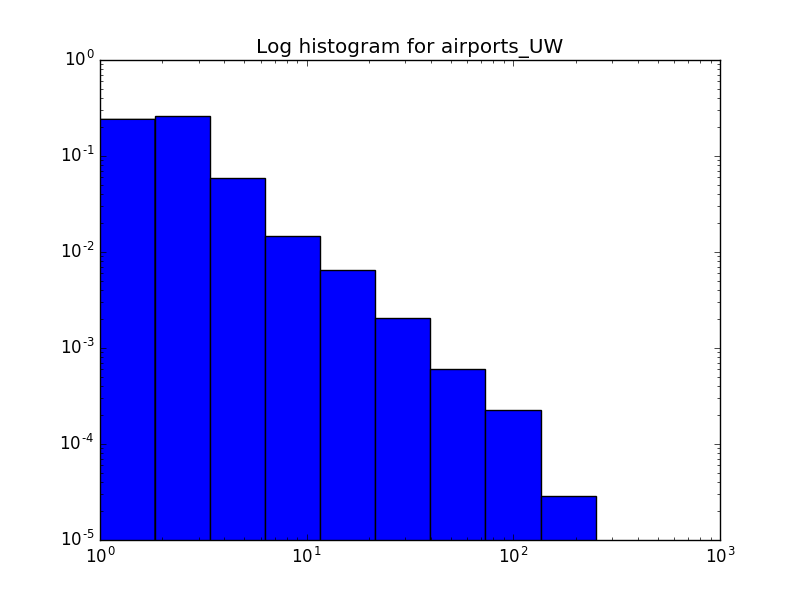
\includegraphics[scale=0.5]{images/log_airports_UW.png}
	\caption{Log scaled histogram for the airports\_UW network.}
	\label{airport}
\end{figure}

\begin{figure}[h!]
	\centering
	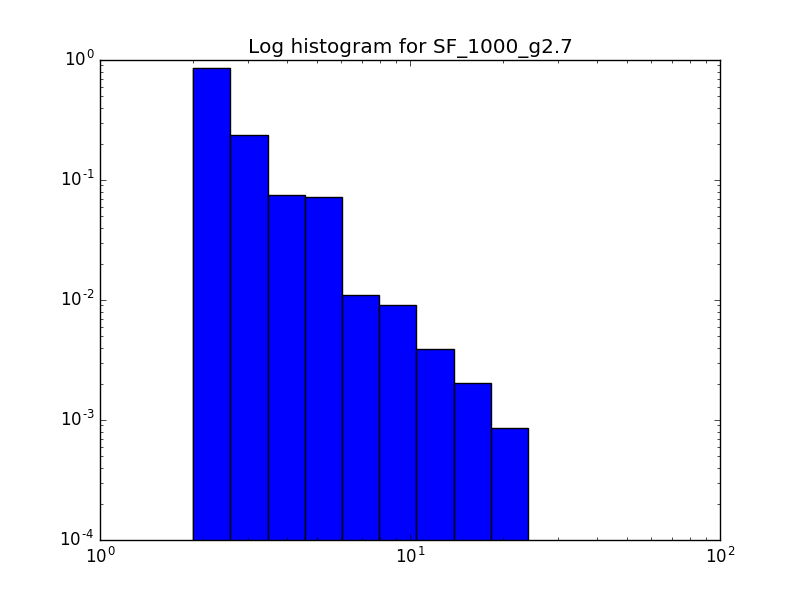
\includegraphics[scale=0.5]{images/log_SF_1000_g2.png}
	\caption{Log scaled histogram for the SF\_1000\_g2.7 network.}
	\label{airport}
\end{figure}

\begin{figure}[h!]
	\centering
	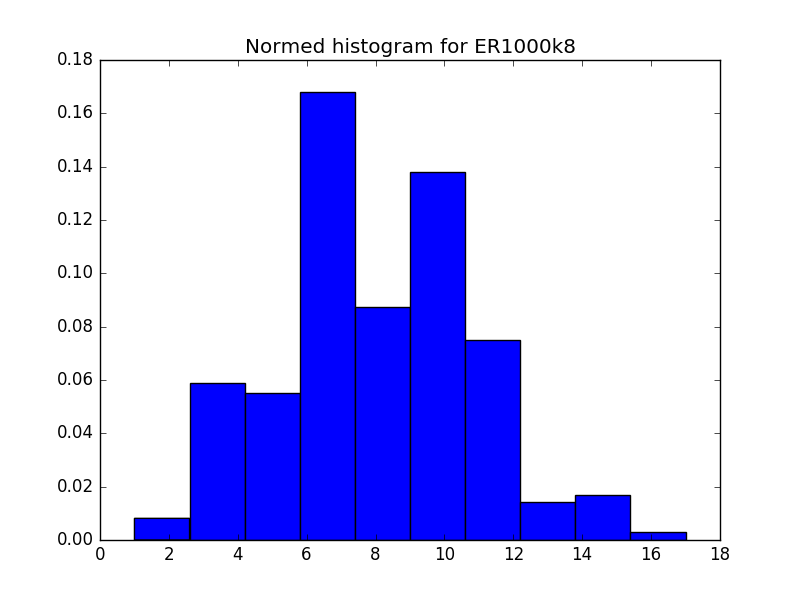
\includegraphics[scale=0.5]{images/norm_ER1000k8.png}
	\caption{Histogram for the ER1000k8 network for probabilities.}
	\label{airport}
\end{figure}

\begin{figure}[h!]
	\centering
	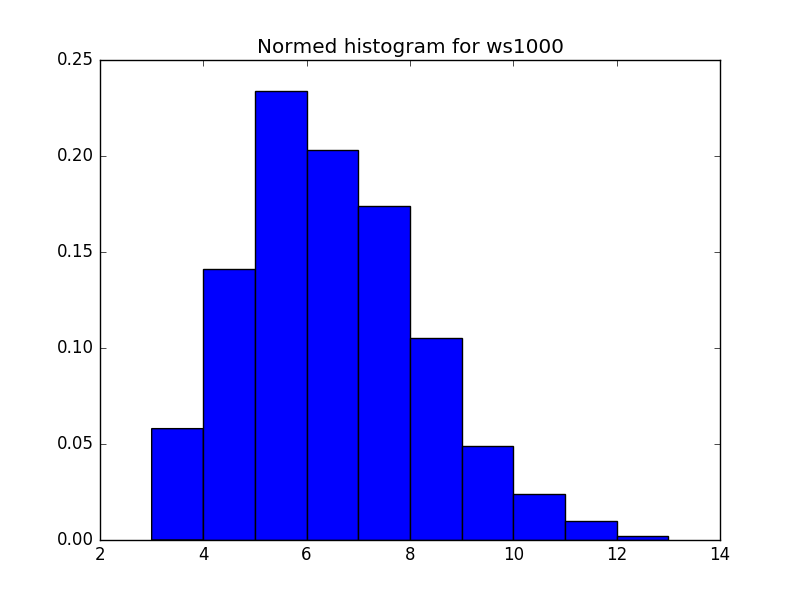
\includegraphics[scale=0.5]{images/norm_ws1000.png}
	\caption{Histogram for the ws1000 network for the probabilies intead of the frecuencies.}
	\label{airport}
\end{figure}

\begin{figure}[h!]
	\centering
	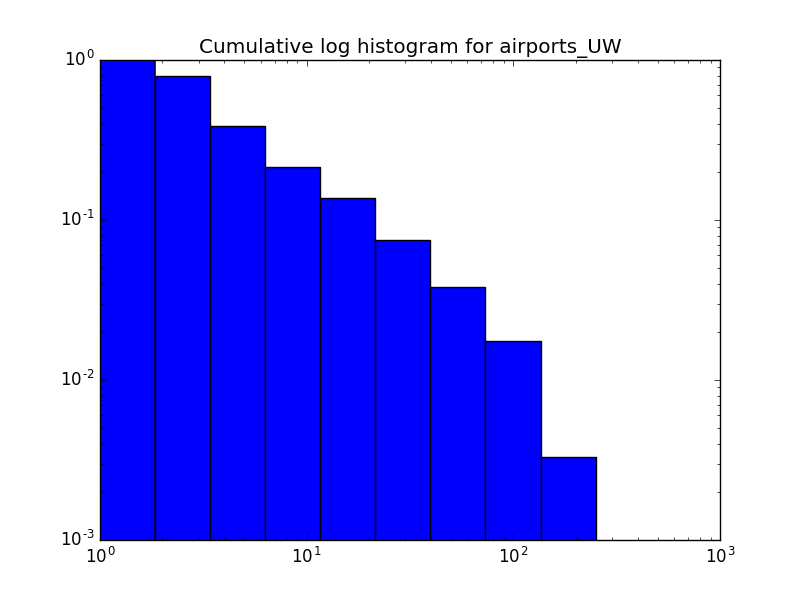
\includegraphics[scale=0.5]{images/Cumu_log_airports_UW.png}
	\caption{Cumulative log scaled histogram for the airports\_UW network.}
	\label{airport}
\end{figure}

\begin{figure}[h!]
	\centering
	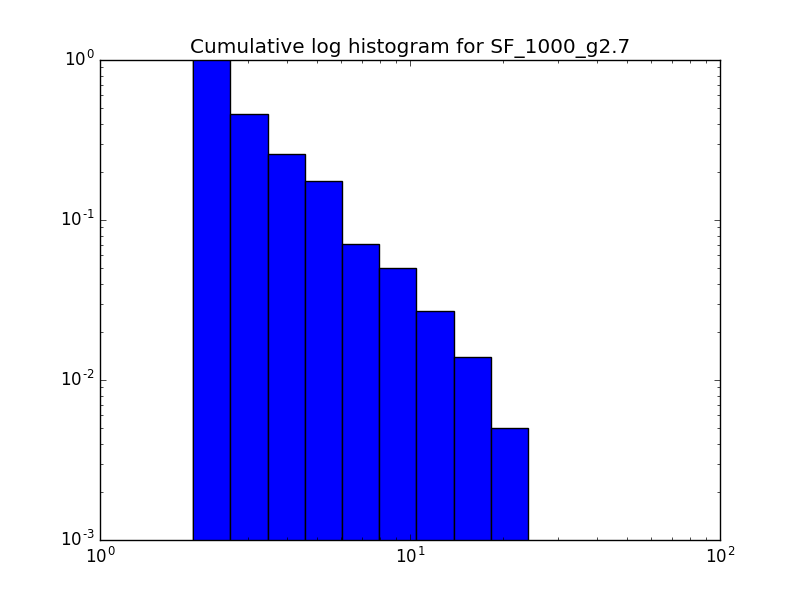
\includegraphics[scale=0.5]{images/Cumu_log_SF_1000_g2.png}
	\caption{Cumulative log scaled histogram for the SF\_1000\_g2.7 network.}
	\label{airport}
\end{figure}

\begin{figure}[h!]
	\centering
	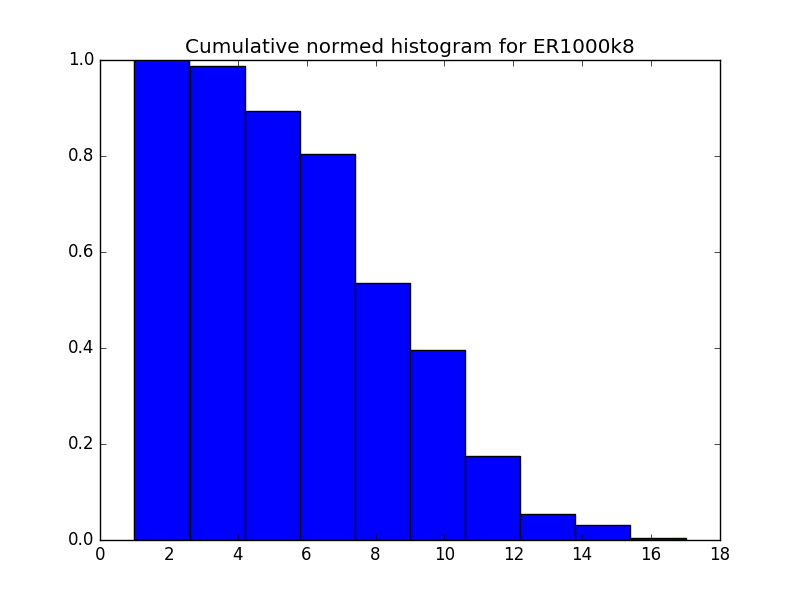
\includegraphics[scale=0.5]{images/Cumu_norm_ER1000k8.png}
	\caption{Cumulative histogram of the probability distribution for ER1000k8 network.}
	\label{airport}
\end{figure}

\begin{figure}[h!]
	\centering
	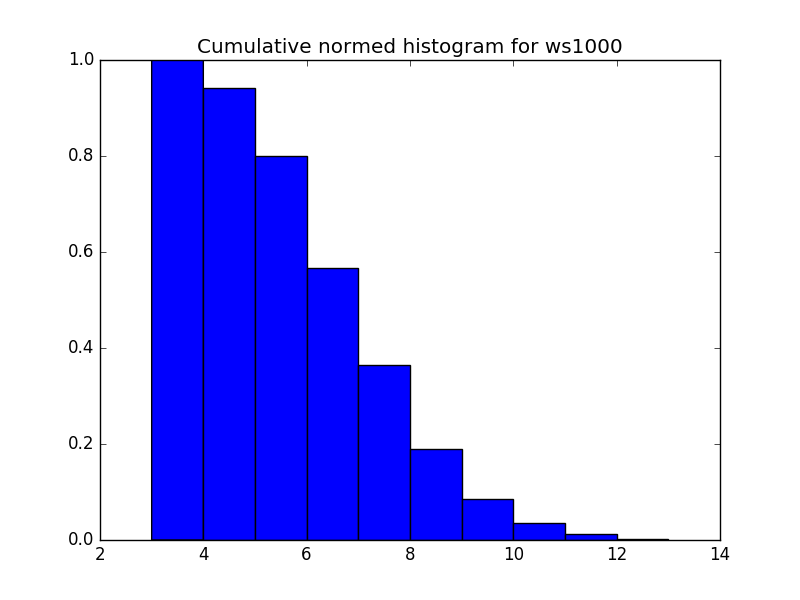
\includegraphics[scale=0.5]{images/Cumu_norm_ws1000.png}
	\caption{Cumulative histogram of the probability distribution for ws1000 network.}
	\label{airport}
\end{figure}

For the networks ER1000k8 and ws100 the usual histogram has been used, with no rescaling, since the distribution can easily be look. For airports\_UW and SF\_1000\_g2.7 networks the histogram has been rescaled to a logarithmic scale for a better representation of the PDF and the CCPDF, in the original version the high connected node can't barely be seen.

\end{document}

